\chapter{Design}

\section{Overall System Design}

\subsection{Short description of the main parts of the system}

Entering new stock: One of the main parts of the system is that it must be able to record inputted data by the user when new stock is to be added to the system. during this prosses the system should display one window into which the user can enter all the data required for the product, this data will then be verifyed before enterd into the database. If the data does not pass verifcation then the user will be told which fields are incorrect and what data should inputted to those fields.

Sending data via email: many parts of the system genarate data that is useful for the pubs management such as all the transactions done by one user in a session. This data will then be sent via email to an external client. The way in wich this will happen is the data will writen to a text file which will then be sent using email to the external client.

recording used stock: The system must be able to keep track of how much stock it has left to do this is must take away stock from the system without deleting the record of the stock from the database. In order to do this every stock item has the atributes stock used and stock remaining, stock used recordes to amount of the stock that has been used either sold or by another means the stock has been used up. Stock remaining does the opersite to this it recordes the amount of stock the system still has. Almost every operation on the system will use these two atributes in one way or another.

refill stock: some stock items will have an display quantity and product displayed atribute; display quantity is the maximum amount of that stock item that can be put on display. product displayed is the real amount of the product that is currently being displayed. the system will uses these atribrutes when a user refills all displayed stock at the end of a session; the system will calcutate how much of each stock is needed and print this on a list. the system will do a simular operation when a items product display reaches a certain value such as 1 or 0.

\subsection{System flowcharts showing an overview of the complete system}

\begin{figure}[H]
    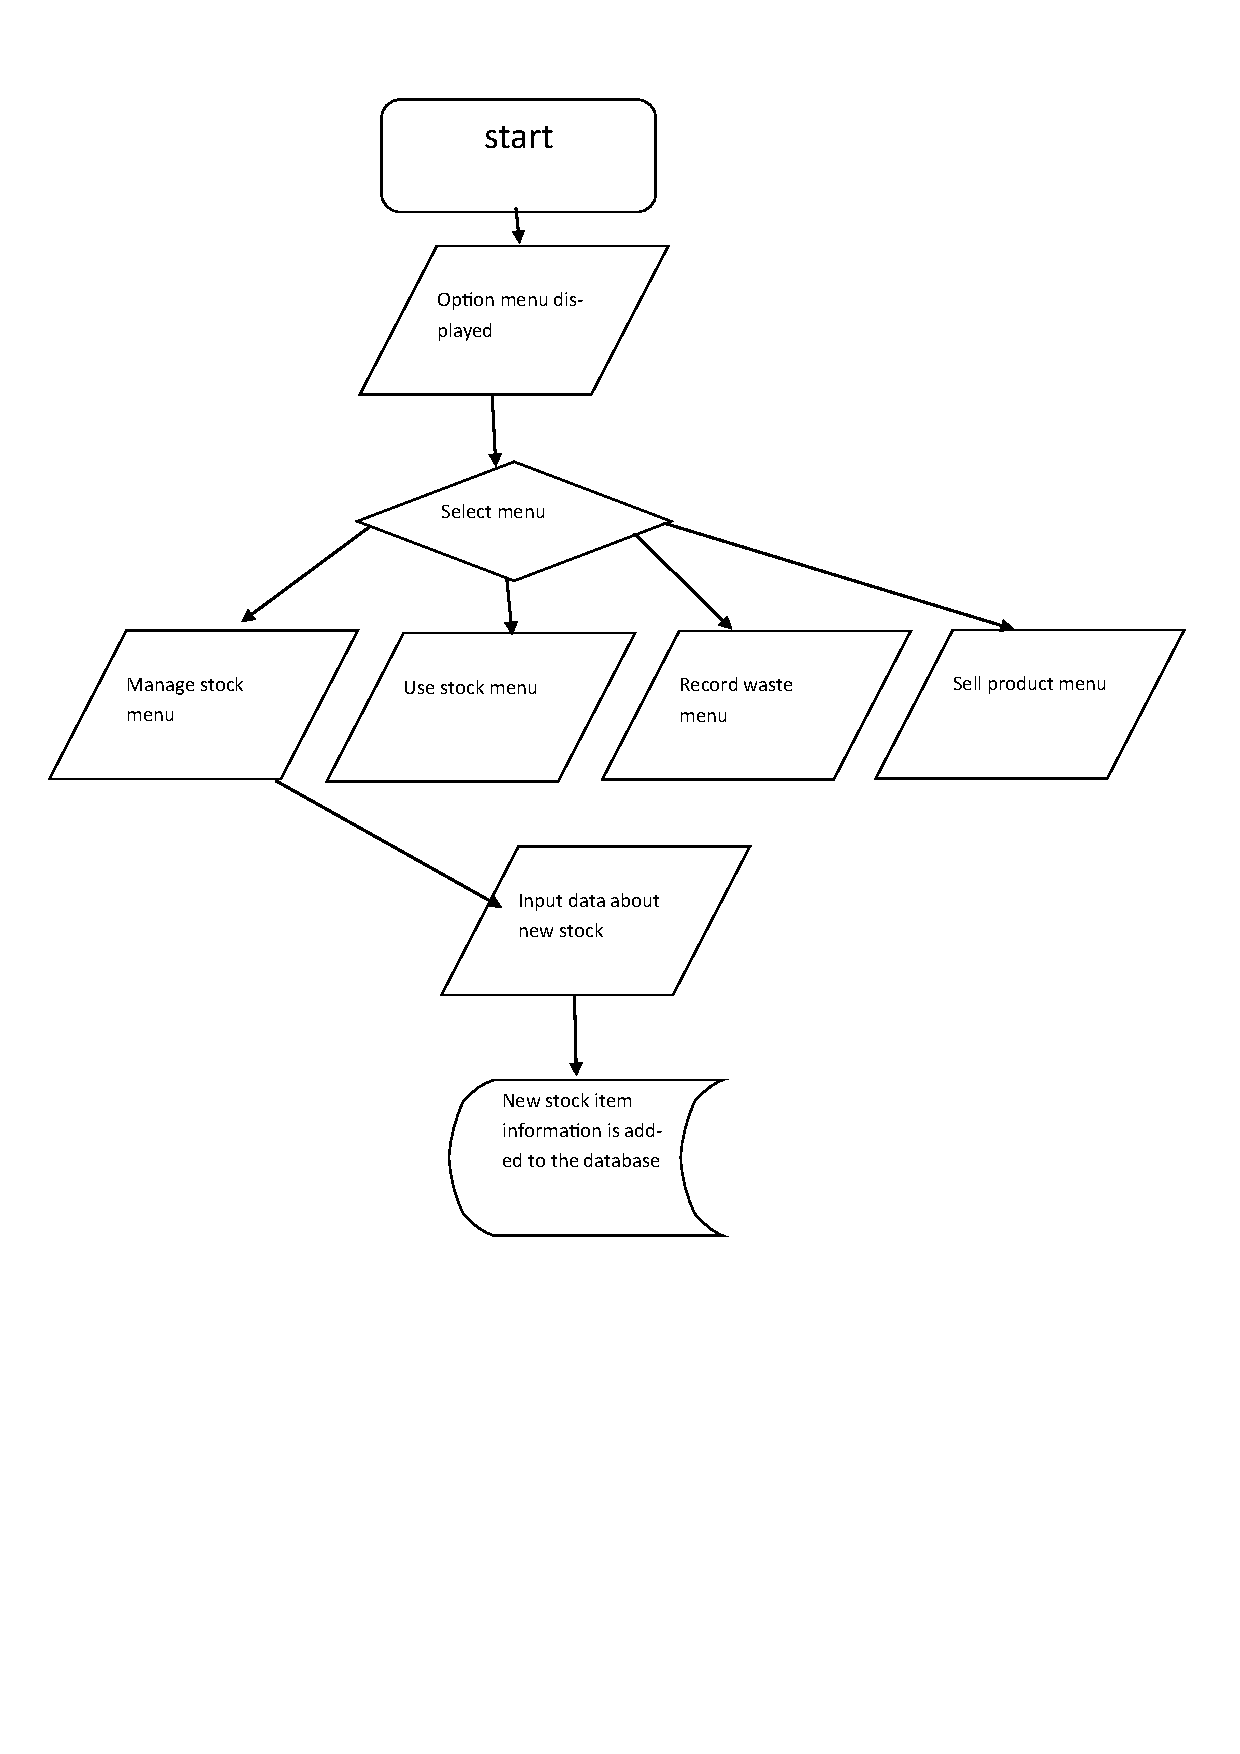
\includegraphics[width=\textwidth]{./Design/pdfimages/flowdiagram_new_stock.pdf}
    \caption{flowdiagram for adding new stock} \label{fig:new stock flowchart}
\end{figure}


\begin{figure}[H]
    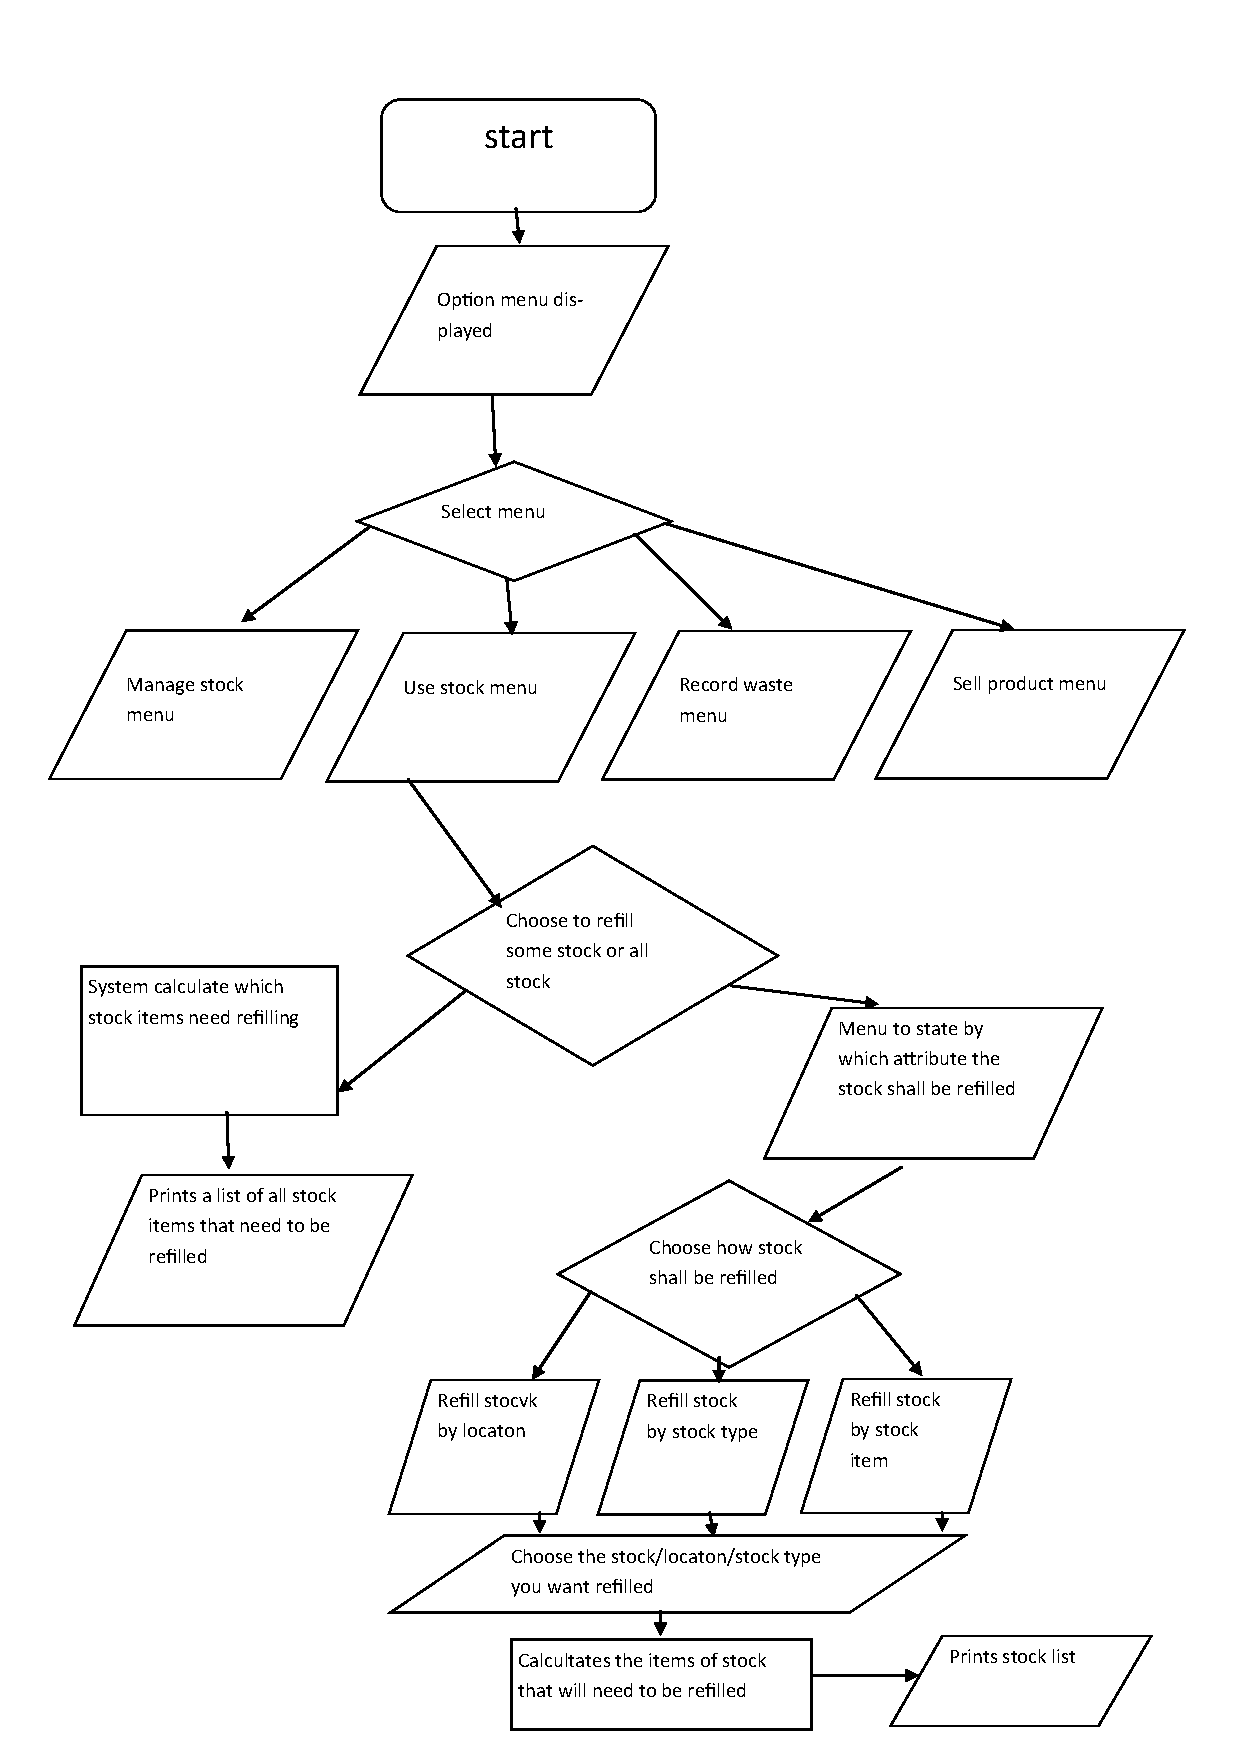
\includegraphics[width=\textwidth]{./Design/pdfimages/flowdiagram_use_stock.pdf}
    \caption{flow diagram use stock} \label{fig:use stock flowdiagram}
\end{figure}

\begin{figure}[H]
    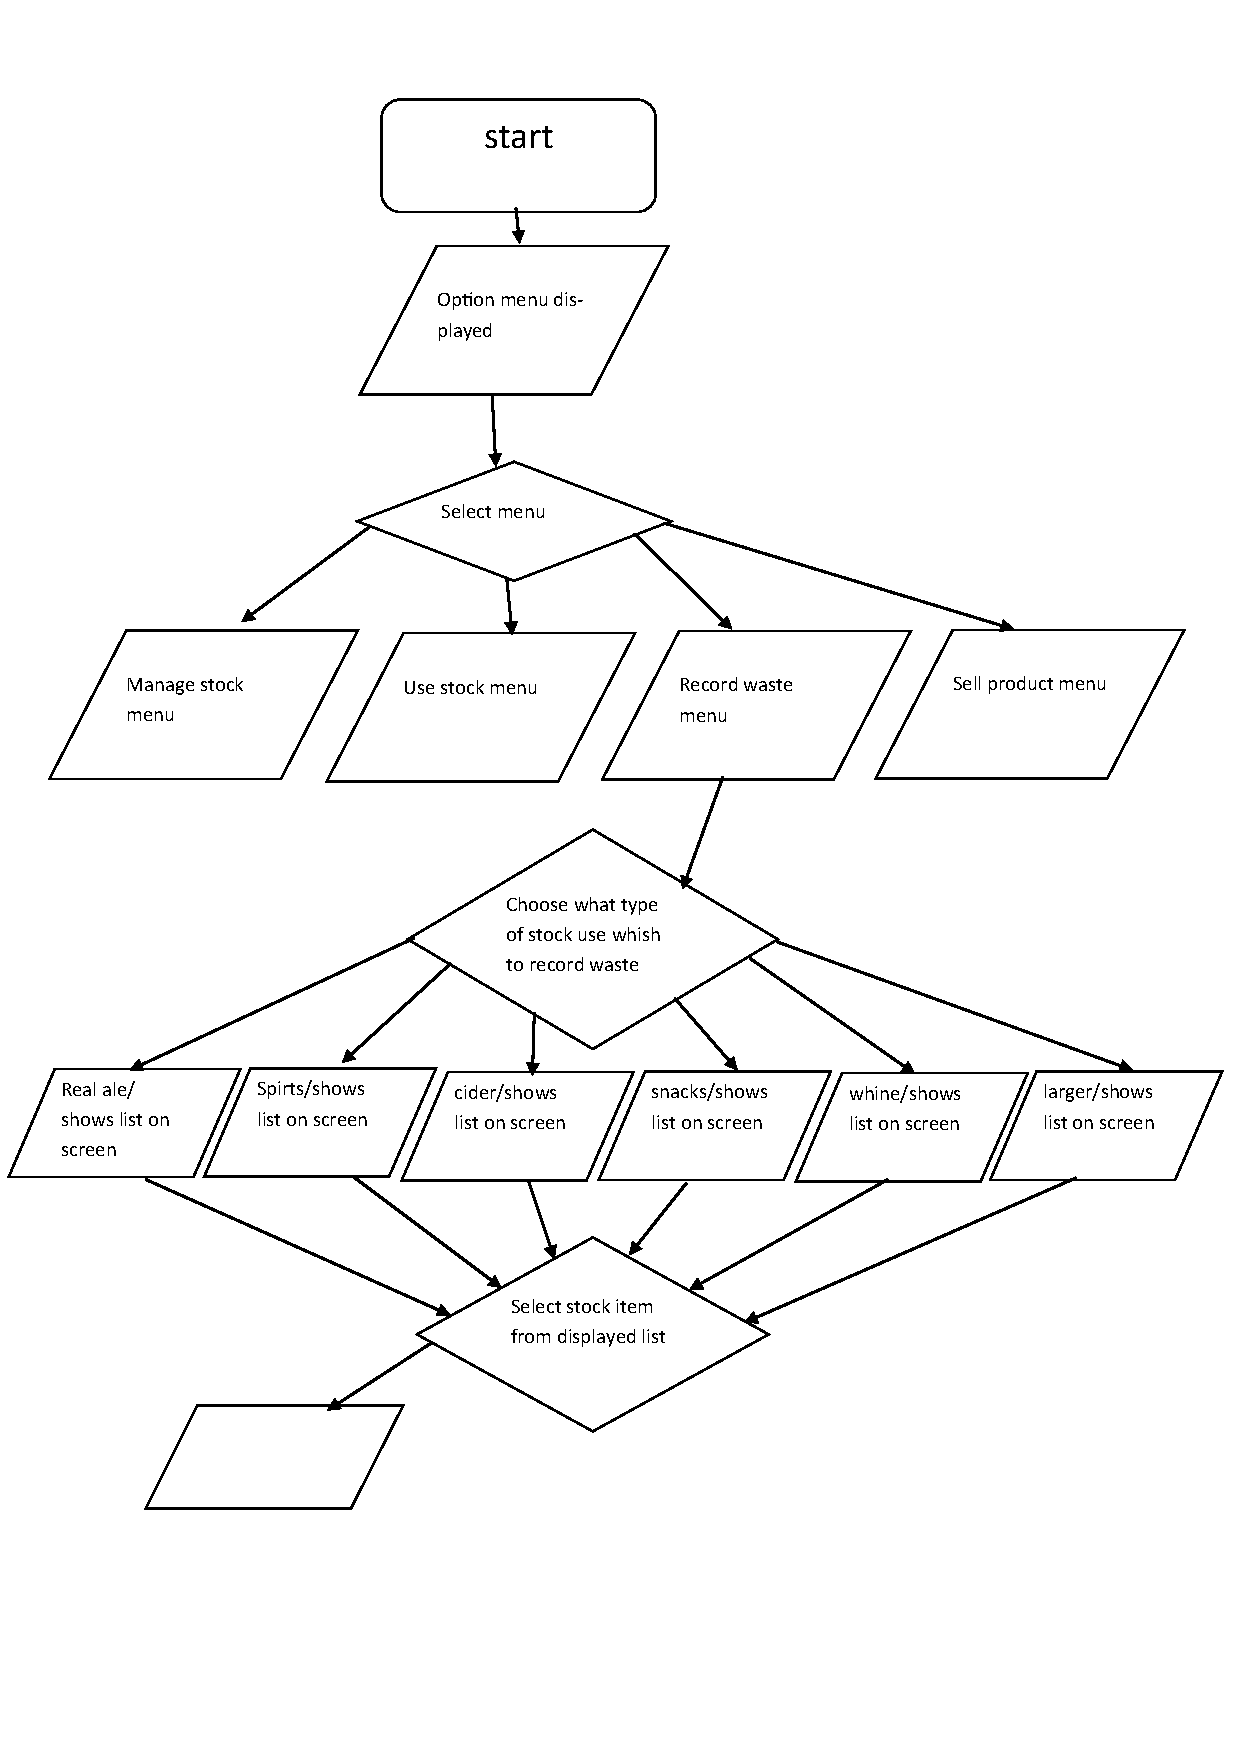
\includegraphics[width=\textwidth]{./Design/pdfimages/flowdiagram_record_waste.pdf}
    \caption{flow diagram for recording waste} \label{fig:record waste flowdiagram}
\end{figure}



\section{User Interface Designs}

\begin{figure}[H]
    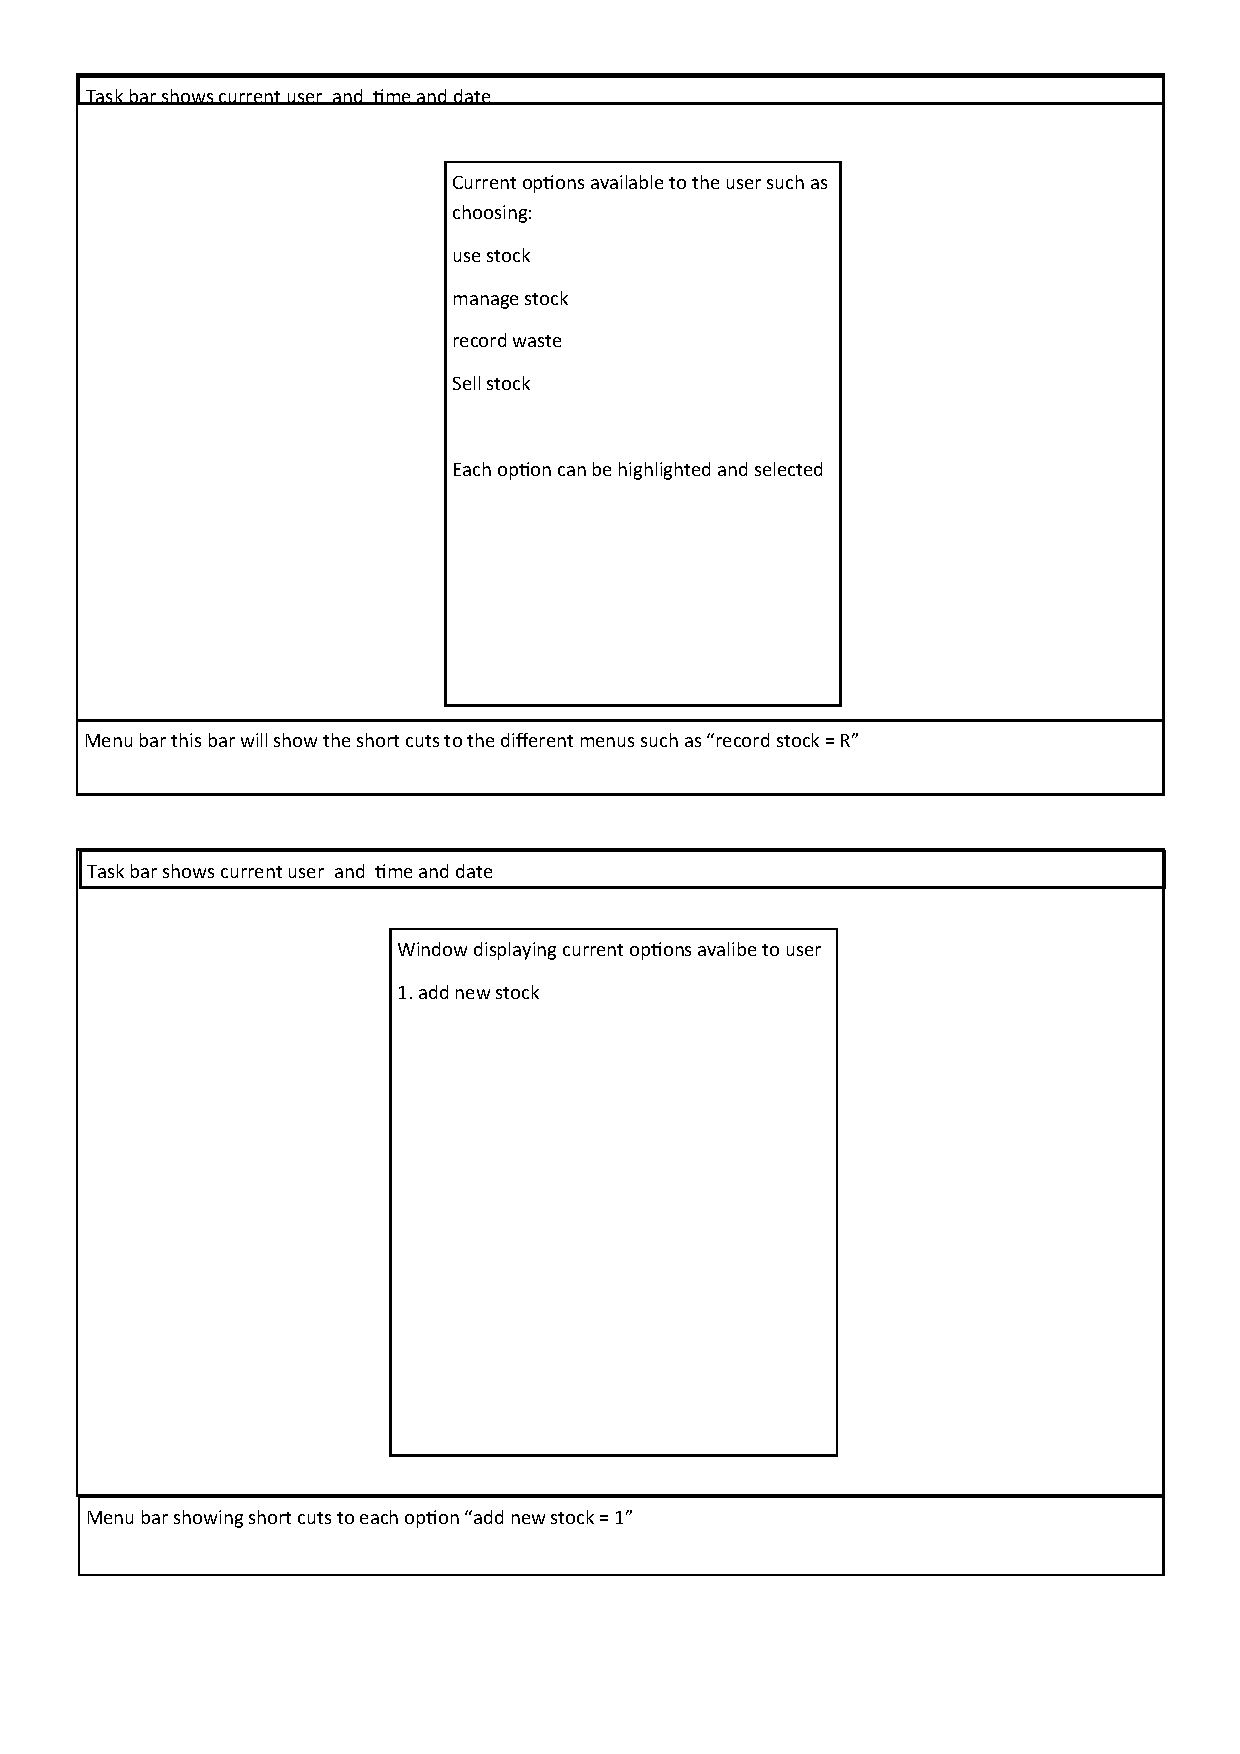
\includegraphics[width=\textwidth]{./Design/pdfimages/gui.pdf}
    \caption{first gui menu} \label{fig:gui homescreen}
\end{figure}



\section{Program Structure}

\subsection{Top-down design structure charts}

\subsection{Algorithms in pseudo-code for each data transformation process}

\subsection{Object Diagrams}

\subsection{Class Definitions}

\section{Prototyping}

\section{Definition of Data Requirements}

\subsection{Identification of all data input items}

\subsection{Identification of all data output items}

\subsection{Explanation of how data output items are generated}

\subsection{Data Dictionary}
\begin{center}
\begin{tabular}{|l|l|l|l|l|l|}
    \hline
    \textbf{Name} & \textbf{Data Type} & \textbf{Length} & \textbf{Validation} & \textbf{Example Data} & \textbf{Comment} \\ \hline
	stock ID & int & 2 bytes & 4 digits, must exsist & 3845 & unique to each stock item\\ \hline
	user ID & int & 2 bytes & 2 digits, must exsist & 04 & unique to each member of staff\\ \hline
	producer & string & 12 bytes & 4-12 chariters & taddingtons & name of product producer\\ \hline
	supplier & string & 14 bytes & 4-14 chariters & milton brewery & name of product supplier \\ \hline
	retail price & float & 2 bytes & int or decimal & 3.10 & price of a product for one base unit\\ \hline
	unit retail & int & 4 bytes & int 1-3 digits & 750 & base unit the product is sold in\\ \hline
	stockname & string & 14 bytes & string 4-14 & dead pony club & name of a product\\ \hline
	unit purchase & int & 3 bytes & int 1-144 & 72 & amount of the product\\ \hline
	unit cost & int & 3 bytes & int 0-150 & 89 & cost of unit purchase\\ \hline
	stock type & string & 8 bytes & 5-8 chariters & real ale & type of stock\\ \hline
	 
\end{tabular}
\label{tab:range_examples}
\end{center}

\subsection{Identification of appropriate storage media}

  


\section{Database Design}

my data base will have 10 tables; users, stock, stock type, real ale, snacks, spirits, unit retail, unit purchase, producer, supplier, permissions.

user (\underline{user ID}, user name, \emph{permissions}, postcode, city, street, house no., landline, mobile no)

stock (\underline{stock ID}, stock name, \emph{stock type}, \emph{unit retail}, retail price, amount used, amount remaining, sell by date, alcohol percentage)

stock type(\underline{stock type ID}, stock type)

producers(\underline{producer ID}, producer)

supplier(\underline{supplier ID}, supplier)

permissions(\underline{permission ID}, permission)

real ale(\underline{real ale ID}, ale name, alcohol percentage, \emph{unit purchase}, \emph{unit retail}, \emph{producer})

snacks(\underline{snack ID}, snack name, \emph{unit purchase}, \emph{unit retail}, \emph{producer})

spirits(\underline{spirts ID}, spirit name, \emph{unit purchase}, \emph{unit retail}, \emph{producer})

larger(\underline{larger ID}, larger name)

unit retail(\underline{unit retail ID}, unit retail)

unit purchase(\underline{unit purchase ID}, unit purchase)

\subsection{Normalisation}






\subsubsection{ER Diagrams}

\subsubsection{Entity Descriptions}

userID; is used to identify each differnt user of the system so that the manegers can look through who did what on the system, we use userID to identify each user as multiple can have the same name.

user name; is used to print the name of the user on screen as well as some documents such as recets

\subsubsection{1NF to 3NF}

\section{Security and Integrity of the System and Data}

\subsection{Security and Integrity of Data}

\subsection{System Security}

\section{Validation}

\section{Testing}

\begin{landscape}
\subsection{Outline Plan}

\begin{center}
    \begin{tabular}{|p{2cm}|p{5cm}|p{5cm}|p{4cm}|}
        \hline
        \textbf{Test Series} & \textbf{Purpose of Test Series} & \textbf{Testing Strategy} & \textbf{Strategy Rationale}\\ \hline
        Example & Example & Example & Example \\ \hline
    \end{tabular}
\end{center}

\subsection{Detailed Plan}

\begin{center}
    \begin{longtable}{|p{1.5cm}|p{2.5cm}|p{2.5cm}|p{2cm}|p{2cm}|p{2cm}|p{2cm}|p{2cm}|}
        \hline
        \textbf{Test Series} & \textbf{Purpose of Test} & \textbf{Test Description} & \textbf{Test Data} & \textbf{Test Data Type (Normal/ Erroneous/ Boundary)} & \textbf{Expected Result} & \textbf{Actual Result} & \textbf{Evidence}\\ \hline
        Example & Example & Example & Example & Example & Example & Example & Example \\ \hline
    \end{longtable}
\end{center}
\end{landscape}